% This line sets the project root file.
% 
% !TEX root = fib2.tex
% 
%------------------------------------------------------------------------------------------------------------%
\documentclass[aps, pra, a4paper, 11pt, nofootinbib, superscriptaddress, tightenlines, 
notitlepage, longbibliography]{revtex4}

% Packages, Macros, Layout, Environments, etc.
% This line sets the project root file.
% 
% !TEX root = ../fib2.tex
% 
%------------------------------------------------------------------------------------------------------------%

%------------------------------------------------------------------------------------------------------------%
% Packages
%------------------------------------------------------------------------------------------------------------%

\usepackage{color}
\usepackage{amsmath,amsfonts,amssymb,amsthm}
\usepackage{graphicx}
\usepackage{fullpage}
%\usepackage{caption}
\PassOptionsToPackage{caption=false}{subfig}
\usepackage{subfig}
\usepackage{enumerate}

\usepackage{tikz}
\usetikzlibrary{arrows,decorations.pathmorphing,backgrounds,positioning,fit}
%\usepackage[square,comma,numbers,sort&compress]{natbib}
\usepackage{epstopdf} % to include .eps graphics files with pdfLaTeX
\usepackage{bm}  % Define \bm{} to use bold math fonts

\usepackage[pdfpagelabels,pdftex,bookmarks,breaklinks]{hyperref}
\definecolor{darkblue}{RGB}{0,0,127} % choose colors
\definecolor{darkgreen}{RGB}{0,150,0}
\hypersetup{colorlinks, linkcolor=darkblue, citecolor=darkgreen, filecolor=red, urlcolor=blue}
%\hypersetup{pdftitle=Title\ Goes\ Here}% add a title to the metadata

\usepackage{layout}

%------------------------------------------------------------------------------------------------------------%
% PGF Stuff
%------------------------------------------------------------------------------------------------------------%

%\pgfrealjobname{main}

%------------------------------------------------------------------------------------------------------------%
% Page Layout
%------------------------------------------------------------------------------------------------------------%

\addtolength{\textheight}{0\textheight}

%------------------------------------------------------------------------------------------------------------%
% Theorem Environments
%------------------------------------------------------------------------------------------------------------%

\newtheorem{theorem}{Theorem}
\newtheorem{proposition}[theorem]{Proposition}
\newtheorem{lemma}[theorem]{Lemma}
\newtheorem{corollary}[theorem]{Corollary}
\newtheorem{definition}[theorem]{Definition}
\newtheorem{remark}[theorem]{Remark}
\newtheorem{example}[theorem]{Example}

\newtheorem{claim}{Claim}[section]

\renewenvironment{proof}[1][Proof]{\noindent\textbf{#1.} }{\ $\Box$}

%------------------------------------------------------------------------------------------------------------%
% Macros
%------------------------------------------------------------------------------------------------------------%

% double-struck math font
\def\N{\mathbb{N}}
\def\Z{\mathbb{Z}}
\def\R{\mathbb{R}}
\def\C{\mathbb{C}}
\def\E{\mathbb{E}}

\def\e{\mathrm{e}}
\def\lg{\mathrm{lg}}

\newcommand{\Eref}[1]{Eq.~(\ref{#1})}
\newcommand{\Sref}[1]{Sec.~\ref{#1}}
\newcommand{\Fref}[1]{Fig.~\ref{#1}}
\newcommand{\Aref}[1]{Appendix~\ref{#1}}

\def\eps{\epsilon}
\def\th{^{\rm th}}
\def\st{^{\rm st}}
\def\rd{^{\rm rd}}
\def\cO{\mathcal{O}}
\DeclareMathOperator{\Tr}{Tr}
\DeclareMathOperator{\tr}{tr}
\DeclareMathOperator{\Prob}{Prob}

\newcommand{\ket}[1]{|{#1}\rangle}
\newcommand{\expect}[1]{\langle{#1}\rangle}
\newcommand{\bra}[1]{\langle{#1}|}
\newcommand{\ketbra}[2]{|{#1}\rangle\!\langle{#2}|}
\newcommand{\braket}[2]{\langle{#1}|{#2}\rangle}
\newcommand{\proj}[1]{\ketbra{#1}{#1}}

%------------------------------------------------------------------------------------------------------------%
% Comment fonts
%------------------------------------------------------------------------------------------------------------%

\newcommand{\cggb}[1]{\textcolor{blue}{#1}}
\newcommand{\sdb}[1]{\textcolor{red}{#1}}


%------------------------------------------------------------------------------------------------------------%
\begin{document}

\title{Classical simulation of error correction in a Fibonacci anyon code}

\author{Simon Burton}
\affiliation{Centre for Engineered Quantum Systems, School of Physics, 
The University of Sydney, Sydney, Australia}
\author{Courtney G.\ Brell}
\affiliation{Institut f\"{u}r Theoretische Physik, Leibniz Universit\"{a}t Hannover, 
Appelstra\ss{}e 2, 30167 Hannover, Germany}
\author{Steven T.\ Flammia}
\affiliation{Centre for Engineered Quantum Systems, School of Physics, 
The University of Sydney, Sydney, Australia}

\date{\today}

\begin{abstract}
We study two-dimensional systems that support Fibonacci anyon excitations. In general, the 
braiding of Fibonacci anyons is sufficient for universal quantum computation, and so the 
classical simulation of their dynamics is likely to be hard. However, we show that for typical 
processes of interest for the study of quantum error correction in anyon systems the 
relevant dynamics can in fact be efficiently simulated classically for a wide range of system 
parameters. We make use of this fact to demonstrate the success of an error-correction 
protocol for a Fibonacci anyon quantum memory below a particular noise threshold. We 
numerically simulate a phenomenological model of the system and noise processes on lattice 
sizes of up to $128\times128$ sites, and demonstrate an error-correction threshold of around 
$12.5\%$, a number that is comparable to those previously known for abelian and 
(non-universal) non-abelian anyon models.
\end{abstract}

\maketitle

%------------------------------------------------------------------------------------------------------------%

%\layout % check the layout

\section{Introduction}


	\cggb{Put introduction back in.}


%------------------------------------------------------------------------------------------------------------%

\section{Modelling Fibonacci anyons}\label{s:model}

	A physical anyon model is abstractly described by a unitary modular tensor category~\cite{?}. This object contains the data describing the types of anyonic particles, as well as the results of topological operations such as braiding or fusion of these anyons. The Fibonacci anyon model consists of only one non-trivial particle type, conventionally called $\tau$. Denoting the vacuum by $\mathbb{I}$, we can describe the possible fusion outcomes of Fibonacci anyons as $\tau\times\tau=\mathbb{I}+\tau$, i.e.~two $\tau$ particles may either fuse to vacuum or to a $\tau$ particle.

	We can associate a Hilbert space with the fusion outcomes of a fixed number of $\tau$ particles, and for $n$ particles of type $\tau$, the dimension of this space grows asymptotically as $\varphi^n$ for $\varphi=\frac{1+\sqrt{5}}{2}$ the golden ratio. Additionally, there is a global degeneracy associated with the topology of the manifold on which the anyons reside. We will consider systems with the topology of a torus, which for the Fibonacci anyons gives rise an extra 2-fold degeneracy. For convenience (in particular to minimize finite-size effects in our numerical computations), this global space is the one in which we will encode, and demonstrate protection of, quantum information.
	
	The fusion outcome of any particular experiment depends on the history of the particles, in particular how they have braided around one another. For this reason braiding operations are considered to act unitarily on the fusion space. Pair-creation events should be considered isometries that enlarge the fusion space, while fusion events correspond to projective measurements of combined charge of some number of particles. For details of the description of these processes in Fibonacci anyons, see Ref.~\cite{?}.

	We use a phenomenological model of Fibonacci anyon dynamics which neglects any microscopic details of the system. This is consistent with the principles of topologically ordered systems and anyonic physics, where the key universal features describing the anyon model correspond to large length-scale physics, while the microscopic physics play a less important and non-universal role. As such, we model the system simply as a square lattice of sites on which sets of anyons may reside. Allowed anyon dynamics are considered to be local on this lattice, which we take to have periodic boundary conditions. For more details of an analogous model, see~\cite{Brell2013}.

	Unlike the Ising anyon systems simulated in Ref.~\cite{Brell2013}, or the $\Phi-\Lambda$ models studied in Refs.~\cite{Wootton2013,Hutter2014}, Fibonacci anyon dynamics are known to be sufficient for universal quantum computation \cite{Freedman2002}. This is because the action of braiding Fibonacci anyons generates a dense set of unitaries on the fusion space (for $n>2$ particles). For this reason, the classsical simulation of such dynamics is expected to be hard in general. As such, it might be expected that the simulation of noise processes and error-correction routines in Fibonacci anyon systems is prohibitively time-consuming. However, we show in \Sref{s:sim} that typical noise processes and error-correction operations may in fact be efficiently simulated on a classical computer in precisely the regimes where we expect error-correction to succeed.
	
%------------------------------------------------------------------------------------------------------------%


\section{Noise and error-correction}\label{s:noise}

	The main noise processes we consider are pair-creation events, in which a pair of $\tau$ anyons are created from vacuum on two neighbouring sites.
	
	\cggb{Details. Consider merging parts of this section with parts of \Sref{s:simalg}.}

	\subsection{Logical errors}
		
		\cggb{Logical operators}

	\subsection{Decoding algorithm}
	
		\cggb{Describe decoding.}

		\cggb{How does this relate to other decoding schemes used in~\cite{Wootton2013,Brell2013,Hutter2014}?}
	
%------------------------------------------------------------------------------------------------------------%	
	
\section{Simulation}\label{s:sim}

	Although simulation of general processes involving $n$ Fibonacci anyons is BQP-complete (and thus unlikely to be classically tractable), noise and error-correction procedures have structure that we can exploit to efficiently simulate typical processes of interest. In particular, those processes in which we expect error-correction to succeed are also those that we expect to be able to efficiently simulate for the following reasons.
	
	Below the (bond) percolation threshold, we expect random sets of bonds to decompose into separate clusters of average size $O(log(n))$ and variance $O(1)$, \cite{Bazant2000}. In our context, the random bonds correspond to noise processes, and so separate clusters correspond to sets of anyons that could not have interacted at any point in their history. As such, we can simulate the braiding processes of each cluster separately. In other words: it is a (tensor) product state, so we compute with each factor separately. Since each cluster has only size $O(log(n))$, we may typically simulate these dynamics efficiently. 
	
	However, random noise processes are not the only dynamics that we need consider. We must also consider the effect of the error-correction routine itself. This acts iteratively to fuse particles on increasing length scales. While this kind of fusion would typically merge clusters, forcing us to compute dynamics of larger and larger sets of anyons, at each length scale the total number of anyons present is dramatically reduced. Indeed, the goal of the error correction algorithm is to reduce the number of anyons as much as possible.
	
	\cggb{Can we make a concrete claim about the maximum size of clusters at each stage of the decoding procedure? Do we know anything about the distribution of separations between clusters in the sub-critical percolation regime?}
	
	Of course, if we were to consider noise so strong that the clusters percolate over the lattice, we would no longer be able to efficiently simulate the system. However, recall that logical errors in our system correspond to processes that act over a non-trivial loop of the torus. If the noise operations are so common to have percolated, this is an example of a situation where we expect error-correction \emph{not} to succeed. Similarly, if the noise has not yet percolated by itself, but the clusters are merged into a large (percolated) cluster by the decoding algorithm, this is again an example of a process that we expect to correspond to a failure of error-correction. So we see that the events that we are able to efficiently simulate correspond precisely to those for which we expect error-correction to succeed. We may simply declare failure on non-simulable events. This allows us to simulate and demonstrate the success of error-correction schemes for Fibonacci anyons, without explicitly simulating the failure of such schemes.

	\subsection{Simulation algorithm}\label{s:simalg}

		We cover the surface of the torus with LxL disjoint squares. These {\it tiles} are the regions over which
charge measurements occur, in order to produce a syndrome for the decoder.

		In order to keep track of the observables of the system we maintain a set of disjoint {\it curves}. These curves can also be thought of as a top-down view of the fusion tree. In general, this winds around the two dimensional tiles in a haphazard way determined by the progress of the simulation. For comparison, previous work used a single fixed Z-shaped curve (row-major ordering) \cite{Brell2013}.

		\begin{center}
		(i)
		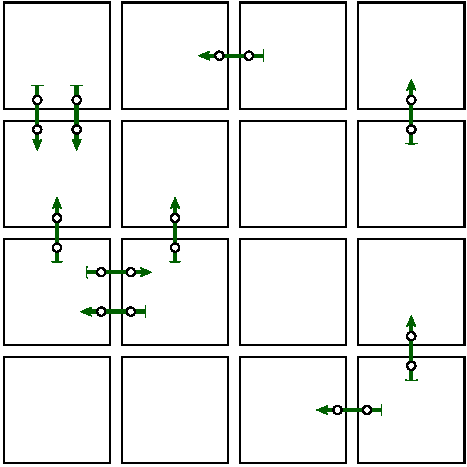
\includegraphics[width=0.26\textwidth]{pair-create.pdf}
		\hskip 10pt
		(ii)
		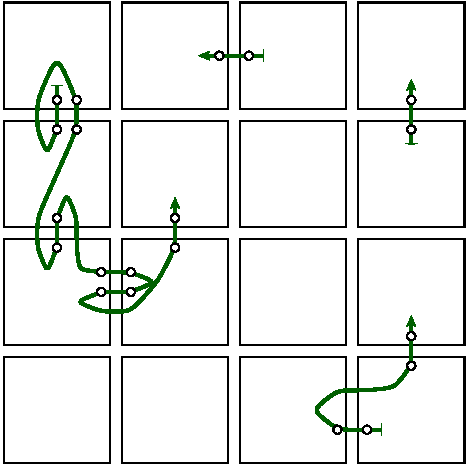
\includegraphics[width=0.26\textwidth]{syndrome-1.pdf}
		\hskip 10pt
		(iii)
		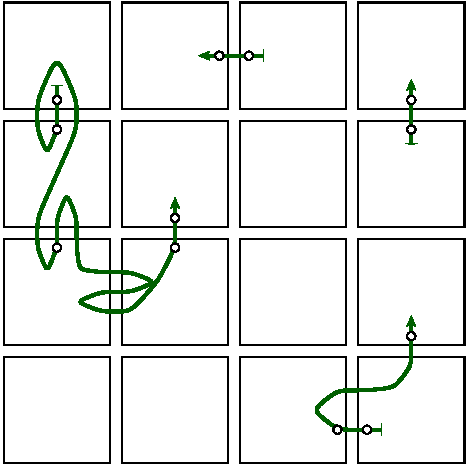
\includegraphics[width=0.26\textwidth]{syndrome-2.pdf}
		\end{center}

		Each round of simulation proceeds in four steps as follows:

		\begin{enumerate}
			\item The noise process is modelled by a sequence of pair-creation events distributed as a Poisson process across each edge.
			\item We first join curves that participate in the same tile in order to,
			\item measure the charge on each tile. Any resulting anyon is left somewhere in the tile.
			\item The decoder examines this syndrome and clusters nearby anyons. Each cluster is then measured (fused), and the decoder continues to cluster and fuse on larger scales until there are no more anyons, or a non-trivial operation has occurred. The non-trivial operations are those that involve a path that wraps around the torus. All of these alter the encoded state, and so in this case we abandon the simulation round and declare failure to error correct. This decoding algorithm is based on the clustering ``RG'' algorithm~\cite{Bravyi2011}.
		\end{enumerate}

%------------------------------------------------------------------------------------------------------------%

\section{Numerical results}

	We plot the performance of the decoder as a function of error rate for varying lattice sizes. The error rate is parameterized by the Poisson process duration $t_{\mathrm{sim}}$. There is clear evidence of a decoding threshold below
which decoding succeeds with asymptotic certainty as the system size increases. This threshold is at $t_{\mathrm{sim}}\simeq 0.125 \pm 0.003.$

	\begin{center}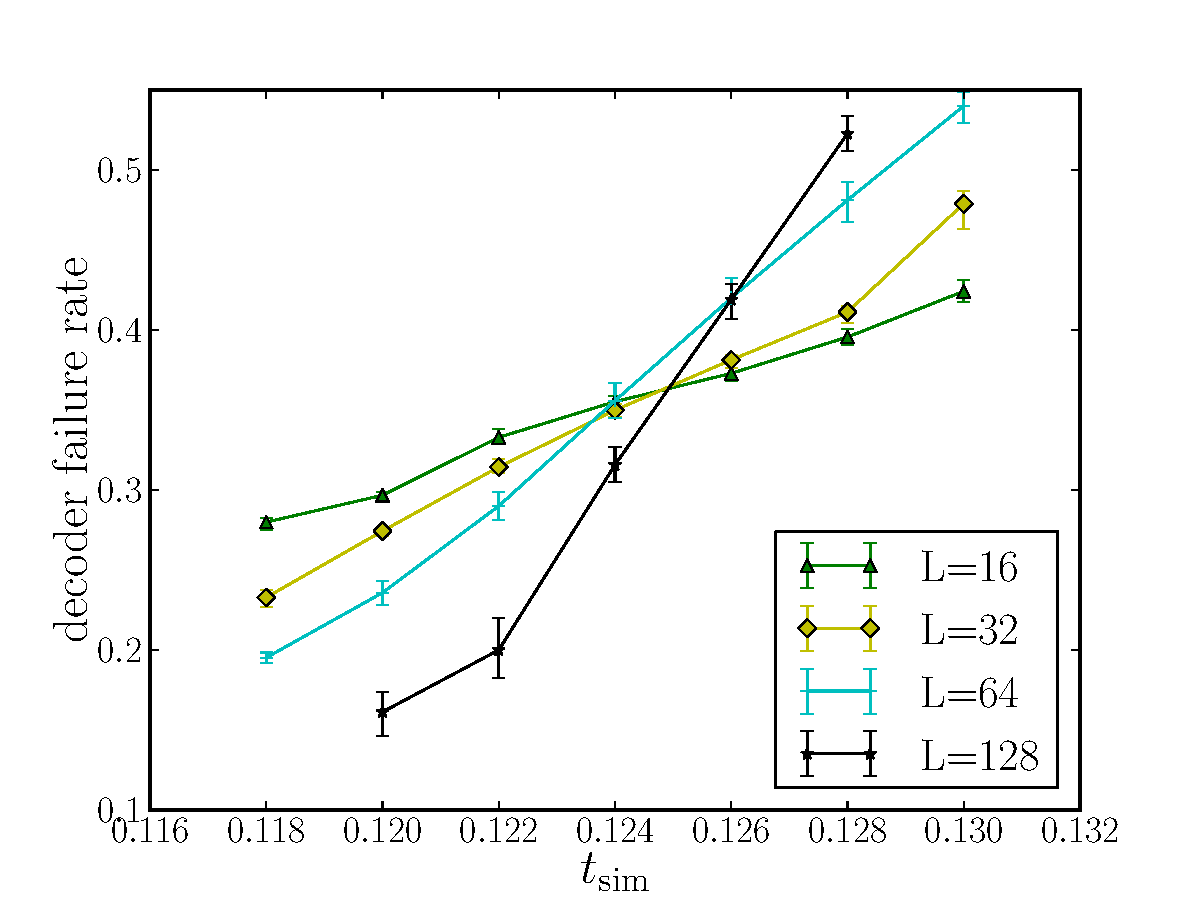
\includegraphics[width=0.6\textwidth]{anyons-kyle.pdf}\end{center}

	\cggb{Define $t_{\mathrm{sim}}$.}
	
	\cggb{Comment on the effect of declaring failure on some simulations on this plot. Would we expect it to change if we simulated every event completely? If so, how?}

%------------------------------------------------------------------------------------------------------------%

\section{Discussion}

	\cggb{Comment on choice of encoding, and applicability of our simulation techniques to simulation of fusion encodings as in Fibonacci anyon computing schemes.}
	
	\cggb{Comment on choice of decoder, noise scheme, etc., particularly noting that the qualitative details are unlikely to be affected by these choices~\cite{Brell2013}.}
	
	\cggb{Comment on the fact that these methods are not restricted to Fibonacci anyons, and could be used to demonstrate the success of error-correction protocols on arbitrary anyon models.}
	
	\cggb{Comment on applicability of our simulation techniques to non-phenomenological models. Is it possible that the same ideas could be useful when there is more microscopic detail available, or are they restricted to exactly our phenomenological setup?}

	\cggb{Do we have much more to say?}

%------------------------------------------------------------------------------------------------------------%
\bibliographystyle{bibstyle}
\bibliography{refs2}

\end{document}
